\chapter{物质中的电磁学}\label{ch:b3:electromagnetism-in-matter}

% Provenance (not for print): completes the "électromagnétisme dans la
% matière" module (dielectrics, magnetism, ferromagnetism) common to the
% surveyed third-year curricula; the Year 2 volume covered only wave
% propagation in media.

在带电电容器的两极板之间插入一片塑料，
电压便随之下降，仿佛电荷凭空出现了一样。在铁钉上绕一圈线圈，
其磁场可增强为原来的一千倍。把装饰磁铁从冰箱上揭下，
它仍“\emph{记得}”自己当初被磁化的方向——
几十年间无需任何电源。本科二年级分册
整体地处理了物质中的场，把材料隐藏在
折射率之中；本章则深入材料内部。本章的思路
电与磁的思路完全相同：物质是大量
微观偶极子的集合，将其求和得到密度（$\vect P$ 或 $\vect M$）；
引入一个辅助场（$\vect D$ 或 $\vect H$），它只关心
我们所能控制的电荷与电流；然后深入到微观尺度
——在\cref{ch:b3:spin-two-level}中的自旋、
\cref{ch:b3:canonical-ensemble}中的玻尔兹曼因子，以及
\cref{ch:b3:phase-transitions}中的平均场相变接手——以计算
材料的行为。本章的结尾在废料场，设计
能吸起汽车的电磁铁。

\section{极化与位移场}

\begin{definition}[极化与束缚电荷]\label{def:b3:electromagnetism-in-matter:polarisation}
\index{极化}\index{束缚电荷}\index{电介质}
\emph{电介质}是分子能够获得（或本身已具有）
电偶极矩的绝缘体。材料的响应由
\emph{极化} $\vect P$ 描述，其定义为单位体积内的偶极矩，
即 $\vect P = n\langle\vect p\rangle$，$n$ 为单位体积内的分子数。
被极化的块体携带\emph{束缚电荷}——
它们不能自由离开，但完全真实：面电荷密度
$\sigma_{\text{b}} = \vect P\cdot\vect n$，位于极化与表面相交处；
以及体电荷密度 $\rho_{\text{b}} =
-\nabla\cdot\vect P$，凡极化不均匀之处即存在。
均匀极化的平板恰等价于两层面电荷 $\pm P$，
分布于两面：其内部偶极子的头尾全部抵消。
\end{definition}

\begin{proposition}[位移场]\label{prop:b3:electromagnetism-in-matter:displacement}
\index{电位移}\index{电极化率}\index{相对介电常数}
总电荷为自由电荷与\omterm{def:b3:electromagnetism-in-matter:polarisation}{束缚电荷}之和，高斯定理中的 $\rho =
\rho_{\text{f}} + \rho_{\text{b}}$ 经整理后化为关于
\emph{\omterm{prop:b3:electromagnetism-in-matter:displacement}{电位移}} $\vect D = \varepsilon_0\vect E +
\vect P$ 的定律：
\[
\nabla\cdot\vect D = \rho_{\text{f}} :
\]
$\vect D$ 的源只有自由电荷——即
极板与导线上的那些电荷。在\emph{线性}\omterm{def:b3:electromagnetism-in-matter:polarisation}{电介质}中，
响应与场成正比，$\vect P = \varepsilon_0\chi_{\text{e}}\vect E$，于是
$\vect D = \varepsilon_0\varepsilon_{\text{r}}\vect E$，其中
$\varepsilon_{\text{r}} = 1 + \chi_{\text{e}}$ 称为\emph{\omterm{prop:b3:electromagnetism-in-matter:displacement}{相对介电常数}}：
空气 $1.0006$、聚乙烯 $2.3$、玻璃 $\sim 5$、
水则高达 $80$。在极板电荷固定的电容器中，
$\vect D$ 不因\omterm{def:b3:electromagnetism-in-matter:polarisation}{电介质}而改变，因此 $\vect E =
\vect D/\varepsilon_0\varepsilon_{\text{r}}$ \emph{减小}为原来的
$\varepsilon_{\text{r}}$ 分之一：束缚面电荷与自由电荷相对，
抵消了其中的大部分场。电容增大为原来的
$\varepsilon_{\text{r}}$ 倍——整个电容器行业
尽在一个希腊字母之中。
\end{proposition}

\begin{proof}
$\nabla\cdot(\varepsilon_0\vect E) = \rho_{\text{f}} +
\rho_{\text{b}} = \rho_{\text{f}} - \nabla\cdot\vect P$；将
\omterm{def:b3:electromagnetism-in-matter:polarisation}{极化}项移至左侧。
\end{proof}

\begin{omfigure}
\begin{tikzpicture}[scale=1.0]
  % capacitor plates
  \fill[gray!30] (-0.25,0) rectangle (0,4);
  \fill[gray!30] (6.2,0) rectangle (6.45,4);
  \draw[thick] (-0.25,0) rectangle (0,4);
  \draw[thick] (6.2,0) rectangle (6.45,4);
  \foreach \y in {0.4,1.2,2.0,2.8,3.6}
    {\node[font=\scriptsize] at (-0.55,\y) {$+$};
     \node[font=\scriptsize] at (6.75,\y) {$-$};}
  % dielectric slab
  \fill[omDef!8] (1.6,0.25) rectangle (4.6,3.75);
  \draw[omDef] (1.6,0.25) rectangle (4.6,3.75);
  % dipoles inside (minus toward left plate's +)
  \foreach \x in {2.15,3.1,4.05}
    \foreach \y in {0.75,1.75,2.75,3.25}
      {\draw[omDef!70] (\x-0.22,\y) -- (\x+0.22,\y);
       \node[omDef, font=\tiny] at (\x-0.3,\y) {$-$};
       \node[omDef, font=\tiny] at (\x+0.3,\y) {$+$};}
  % bound surface charge labels
  \node[omDef, font=\scriptsize, anchor=north] at (1.6,0.15)
    {$-\sigma_{\text{b}}$};
  \node[omDef, font=\scriptsize, anchor=north] at (4.6,0.15)
    {$+\sigma_{\text{b}}$};
  % fields
  \draw[->, thick] (0.3,2) -- (1.3,2) node[midway, above, font=\scriptsize] {$\vect E_0$};
  \draw[->, thick, omDef] (2.4,4.15) -- (3.8,4.15)
    node[midway, above, font=\scriptsize] {$\vect P$};
  \draw[->, thick] (2.8,2) -- (3.4,2) node[midway, above, font=\scriptsize] {$\vect E$};
\end{tikzpicture}

{\small 位于带电极板之间的\omterm{def:b3:electromagnetism-in-matter:polarisation}{电介质}板。电场使分子偶极子定向，
它们内部的电荷两两抵消，
在表面留下束缚面电荷 $\mp\sigma_{\text{b}}$，它们与自由电荷相对，
从而使内部场由 $\vect E_0$ 减小为
$\vect E = \vect E_0/\varepsilon_{\text{r}}$。}
\end{omfigure}

\section{介电常数从何而来}

\begin{proposition}[感应极化与克劳修斯–莫索蒂]\label{prop:b3:electromagnetism-in-matter:mossotti}
\index{极化率}\index{克劳修斯–莫索蒂关系}
处于场 $\vect E_{\text{局域}}$ 中的原子被拉伸为偶极子
$\vect p = \alpha\vect E_{\text{局域}}$，其中 $\alpha$ 为
\emph{\omterm{prop:b3:electromagnetism-in-matter:mossotti}{极化率}}（量纲：$\varepsilon_0\times$体积——
大致为 $\varepsilon_0$ 乘以原子体积）。在稀薄气体中
$E_{\text{局域}} \approx E$，且 $\chi_{\text{e}} =
n\alpha/\varepsilon_0$ 很小。在致密介质中，每个分子还
受到其\omterm{def:b3:electromagnetism-in-matter:polarisation}{极化}的邻居的作用：在其周围挖出一个小球形空腔，
得 $\vect E_{\text{局域}} = \vect E + \vect
P/3\varepsilon_0$，自洽地得到
\emph{\omterm{prop:b3:electromagnetism-in-matter:mossotti}{克劳修斯–莫索蒂关系}}
\[
\frac{\varepsilon_{\text{r}} - 1}{\varepsilon_{\text{r}} + 2}
= \frac{n\alpha}{3\varepsilon_0} :
\]
通过测量蒸气微弱的\omterm{prop:b3:electromagnetism-in-matter:displacement}{电极化率}，即可预言液体的\omterm{prop:b3:electromagnetism-in-matter:displacement}{电极化率}——
对非极性液体，它在百分之几的精度内成立。
\end{proposition}
\admitted

\begin{remark}
此处引用的空腔场 $\vect P/3\varepsilon_0$ 是均匀\omterm{def:b3:electromagnetism-in-matter:polarisation}{极化}%
球体的结果，未加证明；严格的边值
推导属于专门的电动力学课程。上文其余
部分都只是记账。
\end{remark}

\begin{proposition}[极性分子：朗之万函数]\label{prop:b3:electromagnetism-in-matter:langevin}
\index{朗之万函数}\index{取向极化}
具有\emph{固有}偶极矩 $p$ 的分子（水：
$p = \qty{6.2e-30}{C.m}$）无需拉伸——只需取向，
与热运动相抗衡。对
取向求\cref{ch:b3:canonical-ensemble}中的正则平均，能量为
$-pE\cos\theta$，得
\[
\langle\cos\theta\rangle = L(x) = \coth x - \frac1x ,
\qquad x = \frac{pE}{k_{\text{B}}T} ,
\]
称该函数为\emph{\omterm{prop:b3:electromagnetism-in-matter:langevin}{朗之万函数}}：近似线性（$L \approx x/3$），适用于小 $x$。
当场占据绝对优势时饱和于 $1$。在线性区中
$\chi_{\text{e}} = np^2/3\varepsilon_0k_{\text{B}}T$——一种电
居里定律，随 $1/T$ 下降：加热极性液体，其介电常数
\emph{下降}，这一特征用以区分固有偶极子与
感应偶极子。对室温下的水，这一公式预言
$\chi_{\text{e}} \sim 12$——量级正确，氢键
协同作用将实际值推高至 $80$。
\end{proposition}

\begin{proof}[部分证明]
$Z = \int_0^\pi \eu^{x\cos\theta}\,2\pi\sin\theta\,\dd\theta \propto
\sinh x/x$，且 $\langle\cos\theta\rangle = \dd\ln Z/\dd x = \coth x
- 1/x$。展开 $\coth x = 1/x + x/3 - \dots$，对小 $x$ 有
$L \approx x/3$，于是 $P = np\langle\cos\theta\rangle =
np^2E/3k_{\text{B}}T$。
\end{proof}

\begin{omfigure}
\begin{tikzpicture}
  \begin{axis}[omaxis, axis x line=bottom, axis y line=left,
    width=10.4cm, height=5.6cm, xmin=0, xmax=12, ymin=0, ymax=1.15,
    xlabel={$x = pE/k_{\text{B}}T$}, ylabel={$L(x)$},
    xlabel style={at={(axis description cs:0.5,-0.1)}, anchor=north},
    xtick={3,6,9,12}, ytick={1}, clip=true]
    \addplot[gray, dashed, domain=0:12] {1};
    \addplot[omDef, very thick, domain=0.05:12, samples=300]
      {(exp(2*x)+1)/(exp(2*x)-1) - 1/x};
    \addplot[omThm, dashed, thick, domain=0:3.4] {x/3};
    \node[omThm, font=\scriptsize, anchor=west] at (axis cs:2.3,0.55)
      {斜率 $x/3$：居里区};
    \node[gray, font=\scriptsize, anchor=south east] at (axis cs:11.8,1.0)
      {饱和};
  \end{axis}
\end{tikzpicture}

{\small \omterm{prop:b3:electromagnetism-in-matter:langevin}{朗之万函数}。普通场远远处于线性区
（即便在击穿场下 $x \sim 10^{-3}$）：水的偶极子完全取向
需要的场约为
$E \sim \qty{7e8}{V/m}$。}
\end{omfigure}

\section{磁化强度与场 \texorpdfstring{$H$}{H}}

\begin{definition}[磁化强度、束缚电流与 H]\label{def:b3:electromagnetism-in-matter:magnetisation}
\index{磁化强度}\index{磁场 H}\index{磁化率}
磁学的图景与此平行。物质中充满微观的
电流环——绕核运动和自旋的电子，每个都是磁
偶极子 $\vect\mu$；其数密度即\emph{磁化强度}
$\vect M = n\langle\vect\mu\rangle$。一块均匀磁化的块体
等价于沿其侧面环流的\emph{束缚面电流}（内部环流两两抵消；
条形磁铁\emph{就是}一个束缚电流的螺线管）。
把电流分为自由电流与束缚电流，
安培环路定理可围绕辅助场重新写成
\[
\vect H = \frac{\vect B}{\mu_0} - \vect M , \qquad
\oint \vect H\cdot\dd\vect\ell = I_{\text{自由}} :
\]
$\vect H$ 由导线中的电流产生（单位
\unit{A/m}），而 $\vect B$ 保留了物理内容——力、通量、
感应。线性介质满足 $\vect M = \chi_{\text{m}}\vect H$，且
$\vect B = \mu_0(1 + \chi_{\text{m}})\vect H =
\mu_0\mu_{\text{r}}\vect H$。
\end{definition}

\begin{remark}[三种磁性]\label{rem:b3:electromagnetism-in-matter:zoo}
\index{抗磁性}\index{顺磁性}\index{铁磁性}
材料对 $\vect H$ 的响应有三种方式。
\emph{抗磁体}（$\chi_{\text{m}} \sim -10^{-5}$：水、铜、
石墨）的响应类似于将楞次定律永久化：外加场
扰动每个电子轨道，使其反抗外场——响应微弱、普遍存在、
与温度无关，并会被磁铁排斥（曾借此
在 \qty{16}{T} 的孔道中使青蛙悬浮）。
\emph{顺磁体}（$\chi_{\text{m}} \sim +10^{-5}$ 至 $10^{-3}$：
铝、O$_2$）具有固有磁矩——其未配对自旋来自
\cref{ch:b3:identical-particles}——它们像朗之万偶极子那样取向：
$\chi_{\text{m}} = \mu_0 n\mu^2/3k_{\text{B}}T$，居里
$1/T$ 定律（量子两能级版本见
\cref{exo:b3:canonical-ensemble:11}）。
\emph{铁磁体}（铁、钴、镍：$\mu_{\text{r}}$ 达数千）
是自旋之间还相互“通信”的顺磁体——
即\cref{exo:b3:identical-particles:12}所述的交换耦合——
低于\omterm{thm:b3:phase-transitions:meanfield}{居里温度}时，它们\emph{自发}取向：
\cref{thm:b3:phase-transitions:meanfield}，此处正式投入使用。
\end{remark}

\section{铁磁性的应用：磁畴与磁滞}

\begin{definition}[磁畴与磁滞]\label{def:b3:electromagnetism-in-matter:hysteresis}
\index{磁畴}\index{磁滞}\index{剩磁}\index{矫顽场}
原始的铁块\emph{并未}磁化：它碎裂成
\emph{磁畴}，即微米尺度的区域，每个区域内部充分磁化，
但指向各异，因而外部场（及其能量代价）
几乎相互抵消。外加 $\vect H$ 使磁畴壁移动——
有利取向的磁畴增长——随后使整块磁畴转动，
排列一致。磁畴壁会被缺陷钉住，因而过程不可逆：令
$H$ 上下往复变化时，$B(H)$ 描出一条回线，即\emph{磁滞
回线}。切断电流后，仍有\emph{剩磁}场
$B_{\text{r}}$ 保留；要使之归零，需加反向的
\emph{矫顽场}$H_{\text{c}}$。回线所围面积即
每个循环、单位体积耗散的能量。\emph{软磁}
材料（硅钢、铁氧体：回线窄，
$H_{\text{c}}$ 小）用于制作变压器与电动机铁芯；\emph{硬磁}
材料（铝镍钴、Nd$_2$Fe$_{14}$B：回线宽，$H_{\text{c}}$ 极大）用于制成
永磁体，也用于磁存储：冰箱磁铁
与硬盘都是“不肯遗忘”的磁滞回线。
\end{definition}

\begin{omfigure}
\begin{tikzpicture}
  % left: demagnetized domains
  \begin{scope}
    \draw[thick] (0,0) rectangle (3.2,2.4);
    \draw (1.1,0) -- (1.4,2.4);
    \draw (2.2,0) -- (1.9,2.4);
    \draw (0,1.3) -- (1.25,1.15);
    \draw (2.05,1.2) -- (3.2,1.0);
    \draw[->, omDef, thick] (0.45,0.4) -- (0.85,1.0);
    \draw[->, omDef, thick] (1.75,1.9) -- (1.35,1.6);
    \draw[->, omDef, thick] (1.55,0.35) -- (1.85,0.85);
    \draw[->, omDef, thick] (0.4,2.0) -- (0.9,1.75);
    \draw[->, omDef, thick] (2.75,1.9) -- (2.45,1.35);
    \draw[->, omDef, thick] (2.5,0.4) -- (2.9,0.7);
    \node[font=\scriptsize, anchor=north] at (1.6,-0.15)
      {$H = 0$：磁畴相互抵消};
  \end{scope}
  % right: aligned
  \begin{scope}[xshift=5.4cm]
    \draw[thick] (0,0) rectangle (3.2,2.4);
    \foreach \y in {0.5,1.2,1.9}
      {\draw[->, omThm, thick] (0.4,\y) -- (1.4,\y);
       \draw[->, omThm, thick] (1.8,\y) -- (2.8,\y);}
    \node[font=\scriptsize, anchor=north] at (1.6,-0.15)
      {$H$ 较强：单一磁畴};
    \draw[->, thick] (-1.5,1.2) -- (-0.5,1.2)
      node[midway, above, font=\scriptsize] {$\vect H$};
  \end{scope}
\end{tikzpicture}

{\small \omterm{def:b3:electromagnetism-in-matter:hysteresis}{磁畴}。左：原始的铁磁体把磁化隐藏于
相互抵消的区域中。右：外加场增强，并
使\omterm{def:b3:electromagnetism-in-matter:hysteresis}{磁畴}转动，形成单一磁化的整体——经由不可逆的
畴壁跳跃，赋予铁以“记忆”。}
\end{omfigure}

\begin{omfigure}
\begin{tikzpicture}
  \begin{axis}[omaxis,
    width=9.6cm, height=6.4cm, xmin=-3.4, xmax=3.4, ymin=-1.5, ymax=1.5,
    axis lines=middle,
    xlabel={$H$}, ylabel={$B$},
    xtick=\empty, ytick=\empty, clip=false]
    % descending branch (upper): from +sat to -sat
    \addplot[omThm, very thick, domain=-3:3, samples=150]
      {tanh(1.4*(x+0.8))};
    % ascending branch (lower)
    \addplot[omThm, very thick, domain=-3:3, samples=150]
      {tanh(1.4*(x-0.8))};
    % initial magnetization curve
    \addplot[omDef, dashed, thick, domain=0:3, samples=100]
      {tanh(1.05*x)};
    % arrows indicating traversal
    \draw[->, omThm, thick] (axis cs:-0.1,0.752) -- (axis cs:-0.35,0.65);
    \draw[->, omThm, thick] (axis cs:0.1,-0.752) -- (axis cs:0.35,-0.65);
    % remanence and coercivity
    \fill (axis cs:0,0.807) circle (1.5pt);
    \node[font=\scriptsize, anchor=south west] at (axis cs:0.08,0.84)
      {$B_{\text{r}}$};
    \fill (axis cs:-0.8,0) circle (1.5pt);
    \node[font=\scriptsize, anchor=north east] at (axis cs:-0.85,-0.07)
      {$-H_{\text{c}}$};
    \node[omDef, font=\scriptsize, anchor=north west] at (axis cs:1.15,0.62)
      {首次磁化};
    \node[font=\scriptsize, anchor=west] at (axis cs:3.05,0.997)
      {饱和};
  \end{axis}
\end{tikzpicture}

{\small \omterm{def:b3:electromagnetism-in-matter:hysteresis}{磁滞回线}。从原始态（虚线）出发，
场使 $B$ 达到饱和；$H$ 回到零时留下
\omterm{def:b3:electromagnetism-in-matter:hysteresis}{剩磁} $B_{\text{r}}$，只有\omterm{def:b3:electromagnetism-in-matter:hysteresis}{矫顽场}
$-H_{\text{c}}$ 才能将其抹除。回线面积即每循环、单位
体积的热量：变压器用窄回线，永
磁体用宽回线。}
\end{omfigure}

\begin{example}[铁芯电磁铁]\label{ex:b3:electromagnetism-in-matter:electromagnet}
在铁环上绕 $N$ 匝通有电流 $I$ 的线圈，铁环的 $\mu_{\text{r}}
\sim 5000$），环上带有小气隙 $e$。对沿回路的 $\vect H$ 用
安培环路定理：$H_{\text{铁}}\ell + H_{\text{隙}}e = NI$，
且磁通连续，$B$ 处处相同，因此
\[
B\Big(\frac{\ell}{\mu_0\mu_{\text{r}}} + \frac{e}{\mu_0}\Big) = NI .
\]
取 $\ell = \qty{1}{m}$，$e = \qty{1}{cm}$，则气隙项为
铁芯项的五十倍：线圈几乎全部的努力都用于
把磁场推过一厘米的空气。这便是磁路的要点：铁是近乎
完美的磁通导体，空气则相当于“电阻器”，
因而电动机、继电器和废料场起重磁铁
都力求把气隙做得尽可能薄
（见\cref{pb:b3:electromagnetism-in-matter:1}）。
\end{example}

\begin{omfigure}
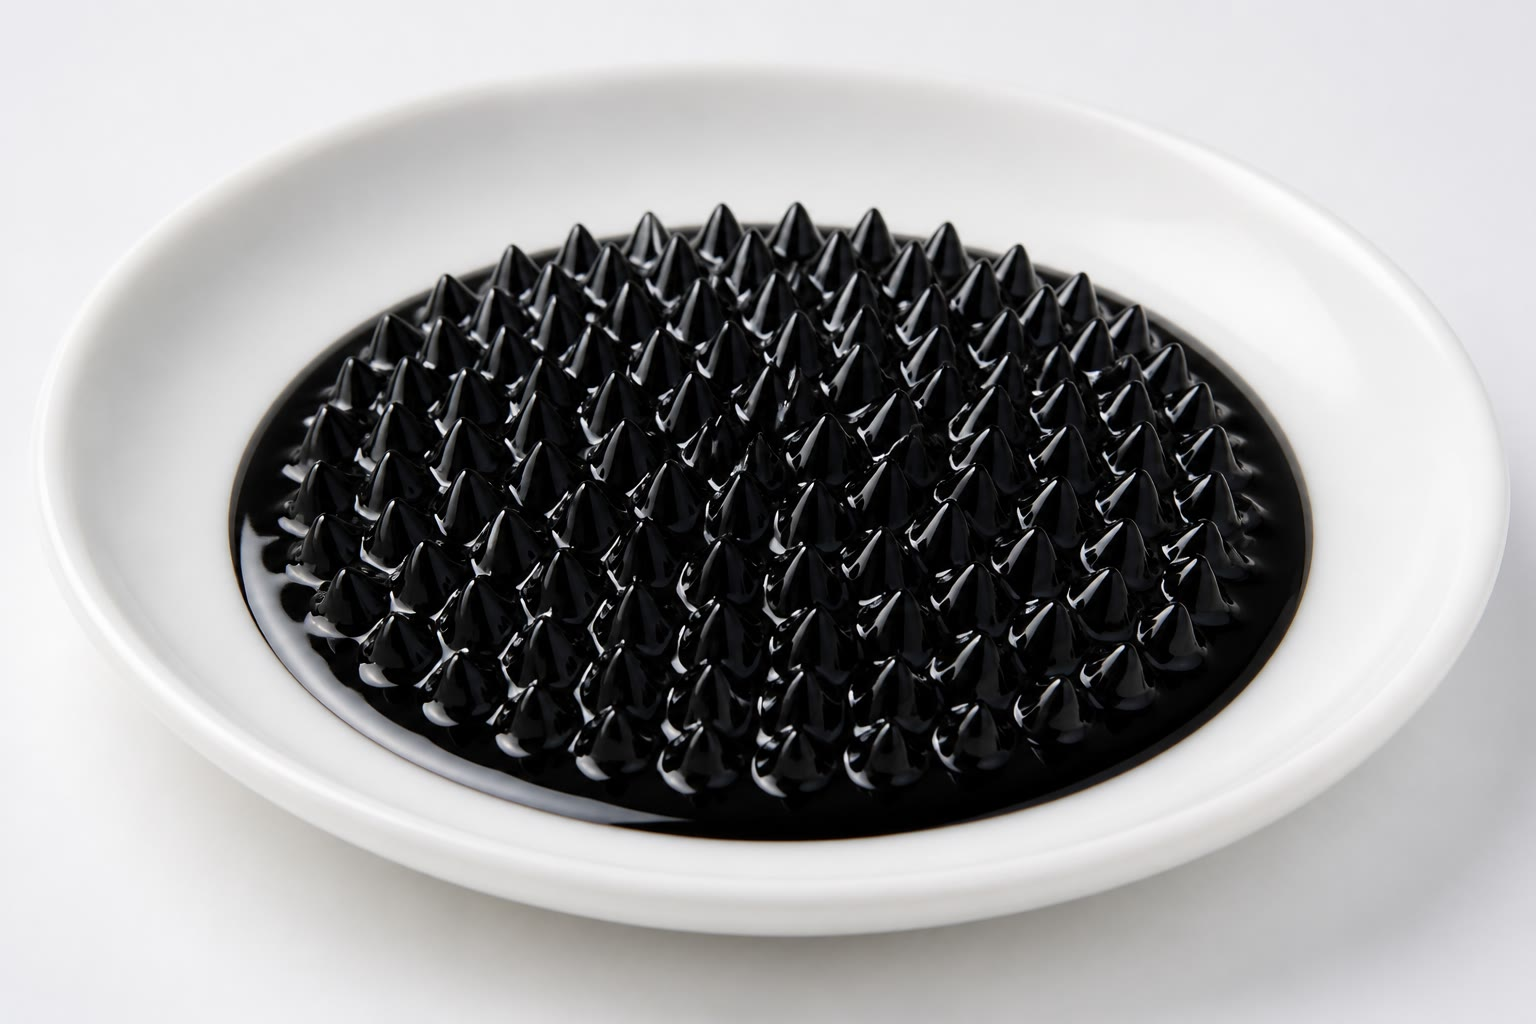
\includegraphics[width=0.58\linewidth]{images/book5/ai/b5-18-ferrofluid-spikes.jpg}

{\small 隐藏磁铁上方的磁流体：液体的磁化使场能的代价低于重力和表面张力，液面于是隆起成尖刺点阵——即可见的 $\vect M$。}
\end{omfigure}

\section{练习}

\begin{exercise}[$\star$]\label{exo:b3:electromagnetism-in-matter:1}
\omterm{def:b3:electromagnetism-in-matter:polarisation}{束缚电荷}的核算。厚度为 $d$ 的平板
沿法线方向均匀\omterm{def:b3:electromagnetism-in-matter:polarisation}{极化}，\omterm{def:b3:electromagnetism-in-matter:polarisation}{极化}强度大小为 $P$。(a) 给出各表面上的\omterm{def:b3:electromagnetism-in-matter:polarisation}{束缚
电荷}面密度。(b) 证明：由这些面电荷产生的\emph{内部}场
为 $E = P/\varepsilon_0$，方向与 $\vect P$ 相反。(c)
若全空间无自由电荷，求内部的 $\vect D$。(d) 一根条形
驻极体（冻结的 $\vect P$）相当于电学中的
哪种磁学对象？
\end{exercise}

\begin{exercise}[$\star$]\label{exo:b3:electromagnetism-in-matter:2}
含\omterm{def:b3:electromagnetism-in-matter:polarisation}{电介质}的电容器。一个平行板电容器
（$C_0 = \qty{100}{pF}$）充电至 \qty{12}{V} 后断开电源。
一块 $\varepsilon_{\text{r}} = 4$ 的平板充满其间。求 (a) 新的
电容；(b) 新的电压；(c) 前后的能量，
——能量差去了哪里？(d) 在电池保持连接的情况下，
重做 (b)–(c)。
\end{exercise}

\begin{exercise}[$\star$]\label{exo:b3:electromagnetism-in-matter:3}
\omterm{def:b3:electromagnetism-in-matter:magnetisation}{磁化率}大观。判断（抗磁、顺磁或铁磁）属于哪一类，
并在可能时由电子结构加以说明：水
（$\chi_{\text{m}} = -9\times10^{-6}$）、铝
（$+2.2\times10^{-5}$）、液氧（$+3.5\times10^{-3}$——
为何 O$_2$ 竟具有磁性？）、镍（$\mu_{\text{r}} \sim 600$
弱场下）。四者中哪些会被强磁铁明显吸引，
哪些则会被微弱排斥？
\end{exercise}

\begin{exercise}[$\star$]\label{exo:b3:electromagnetism-in-matter:4}
$B$、$H$、$M$。一根长螺线管（$n = \num{2000}$ 匝/米，
$I = \qty{1.5}{A}$）内充满铁，测得 $B = \qty{1.6}{T}$。
求 (a) $H$；(b) $M$；(c) 放大倍数
$B/\mu_0H$；(d) 与 $M$ 等效的每米束缚面电流，
并与线圈自身的 $nI$ 比较。
\end{exercise}

\begin{exercise}[$\star\star$]\label{exo:b3:electromagnetism-in-matter:5}
同轴电缆，绝缘。一根同轴线（内半径 $a$，外
半径 $b$），内芯上单位长度带有自由电荷 $\lambda$，
其间充以\omterm{prop:b3:electromagnetism-in-matter:displacement}{相对介电常数}为 $\varepsilon_{\text{r}}$ 的\omterm{def:b3:electromagnetism-in-matter:polarisation}{电介质}。(a) 由对称性求
$\vect D(r)$。(b) 推出 $\vect E$ 与 $\vect P$。
(c) 计算 $r = a$ 与 $r = b$ 处的\omterm{def:b3:electromagnetism-in-matter:polarisation}{束缚电荷}面密度，
并验证单位长度上二者之和为零。(d) 证明单位长度的电容
变为原来的 $\varepsilon_{\text{r}}$ 倍。
\end{exercise}

\begin{exercise}[$\star\star$]\label{exo:b3:electromagnetism-in-matter:6}
克劳修斯–莫索蒂公式的应用。气态氩在 \qty{1}{bar}、
\qty{300}{K} 下的 $\varepsilon_{\text{r}} = 1.00052$。(a) 求出 $\alpha/\varepsilon_0$（一个体积量），
并与原子体积作比较。(b) 液氩的 $n = \qty{2.1e28}{m^{-3}}$，
由克劳修斯–莫索蒂公式预言 $\varepsilon_{\text{r}}$
（实测值 1.53）。
(c) 为何朴素的 $\chi = n\alpha/\varepsilon_0$ 在此处
高估远不如水那样严重？(d) 对哪些分子
整个方案必然失效，又由什么取代？
\end{exercise}

\begin{exercise}[$\star\star$]\label{exo:b3:electromagnetism-in-matter:7}
水的巨大介电常数。(a) 由
\cref{prop:b3:electromagnetism-in-matter:langevin}，计算
水的 $\chi_{\text{e}} = np^2/3\varepsilon_0k_{\text{B}}T$，
（$n = \qty{3.3e28}{m^{-3}}$，$p = \qty{6.2e-30}{C.m}$，
$T = \qty{300}{K}$）。(b) 估算使 $x = 1$（严重饱和）所需的场，
并与水的介电强度相比较，
$\sim\qty{7e7}{V/m}$。(c) 微波炉工作频率为 \qty{2.45}{GHz}，
为何\emph{有损耗的}转动偶极子响应会加热食物，
为何冰的加热速度远慢于液态水？(d) 预言
$\dd\varepsilon_{\text{r}}/\dd T$ 的符号，对水与
氩分别如何？
\end{exercise}

\begin{exercise}[$\star\star$]\label{exo:b3:electromagnetism-in-matter:8}
抗磁性的估算。将原子中的电子视为位于一个
半径为 $r$ 的环上的电荷；外加 $B$ 使其角频率改变拉莫尔频移
$\Delta\omega = eB/2m_{\text{e}}$。(a) 证明感应磁矩
为 $\Delta\mu = -e^2r^2B/4m_{\text{e}}$（与
$B$）反向。(b) 对取向求平均，并对每个原子的 $Z$ 个电子求和，
得 $\chi_{\text{m}} = -\mu_0ne^2Z\langle
r^2\rangle/6m_{\text{e}}$，对水计算（$n =
\qty{3.3e28}{m^{-3}}$ 个分子，$Z = 10$，$\langle r^2\rangle
\approx (\qty{0.7}{\angstrom})^2$），并与实测值
$-9\times10^{-6}$ 相比较。(c) 为何抗磁性与温度无关，
而顺磁性并非如此？(d) 为何连青蛙都能在
\qty{16}{T} 中悬浮，且磁体的场为何必须是\emph{非均匀}的？
\end{exercise}

\begin{exercise}[$\star\star$]\label{exo:b3:electromagnetism-in-matter:9}
居里顺磁性与冷却。某种盐含有 $n =
\qty{2e27}{m^{-3}}$ 的离子，磁矩 $\mu \approx \mu_{\text{B}}$。
(a) 计算 $\chi_{\text{m}} = \mu_0n\mu^2/3k_{\text{B}}T$ 在
\qty{300}{K} 与 \qty{1}{K} 时的值。(b) 在何温度下
$\chi_{\text{m}}$ 达到 $1$——哪种（此处忽略的）物理
会在大多数盐中率先介入？(c) 绝热退磁：
在 \qty{1}{K} 下磁化，隔绝，然后缓慢撤去场——
借助自旋熵，
在\cref{ch:b3:microcanonical-ensemble}中解释样品为何降温。(d)
为何该方法需要\emph{顺}磁体而非铁磁体？
\end{exercise}

\begin{exercise}[$\star\star\star$]\label{exo:b3:electromagnetism-in-matter:10}
磁路。一个铁制环形磁芯（$\ell = \qty{60}{cm}$，
$\mu_{\text{r}} = 4000$，\omterm{def:b3:scattering-theory:cross-section}{截面}积 $A = \qty{16}{cm^2}$），绕有
$N = 500$ 匝，并有一气隙 $e = \qty{4}{mm}$。(a) 证明 $NI =
B(\ell/\mu_0\mu_{\text{r}} + e/\mu_0)$，并计算
$B = \qty{1.2}{T}$ 时的电流。(b) 在 $NI$ 中，用于气隙的占比是多少？
(c) 定义各段的磁阻 $\mathcal R = \ell/\mu A$，
并将 (a) 改写为磁通的串联“欧姆定律”。(d)
铁在 \qty{1.8}{T} 附近饱和：试说明
超过该值后，磁路模型——以及你的电动机——会发生什么变化。
\end{exercise}

\begin{exercise}[$\star\star\star$]\label{exo:b3:electromagnetism-in-matter:11}
\omterm{def:b3:electromagnetism-in-matter:hysteresis}{磁滞}损耗。一台变压器的铁芯（体积 \qty{4e-3}{m^3}）
工作频率为 \qty{50}{Hz}。其硅钢\omterm{def:b3:electromagnetism-in-matter:hysteresis}{磁滞回线}每周期所包围的
能量密度为 $\sim\qty{40}{J/m^3}$。(a) 计算\omterm{def:b3:electromagnetism-in-matter:hysteresis}{磁滞}功率
损耗。(b) 若同一铁芯改用硬钢
（$\sim\qty{6e3}{J/m^3}$），求其损耗并作判断。(c) 涡流附加
一项 $\propto f^2$ 的损耗：试说明铁芯为何做成叠片，以及为何
在射频频段改用铁氧体。(d) 硬盘中的一个比特须
在十年间\emph{保持}其磁化状态，以抵抗热扰动：
请将存储器对 $H_{\text{c}}$ 的要求与变压器的要求相比较，
并由此得出结论：没有任何单一材料能同时胜任这两项工作。
\end{exercise}

\begin{exercise}[$\star\star\star$]\label{exo:b3:electromagnetism-in-matter:12}
退磁场。在无自由电流、均匀磁化的物体内部，
$\oint\vect H\cdot\dd\vect\ell = 0$ 迫使
内部的 $\vect H$ 须\emph{反向}于 $\vect M$（$\vect H =
-N_{\text{d}}\vect M$，其中 $N_{\text{d}}$ 为形状因子：球体取 $1/3$，
沿长针方向 $\approx 0$，垂直于
薄板方向 $\approx 1$）。(a) 借助
束缚电流（螺线管）图像论证针状与薄板两种极限。(b) 为何短粗的磁铁
会部分自退磁，而针状磁体却能保持其
磁化状态？(c) 联系指南针以及磁带中细长的
磁颗粒。(d) 一个软铁球置于均匀的
外磁场 $B_0$ 中：试说明为何其响应在 $\vect H
\approx 0$ 时饱和，即内部 $M \approx 3B_0/\mu_0$ 至多，无论
$\mu_{\text{r}}$ 多大。
\end{exercise}

\begin{omfigure}
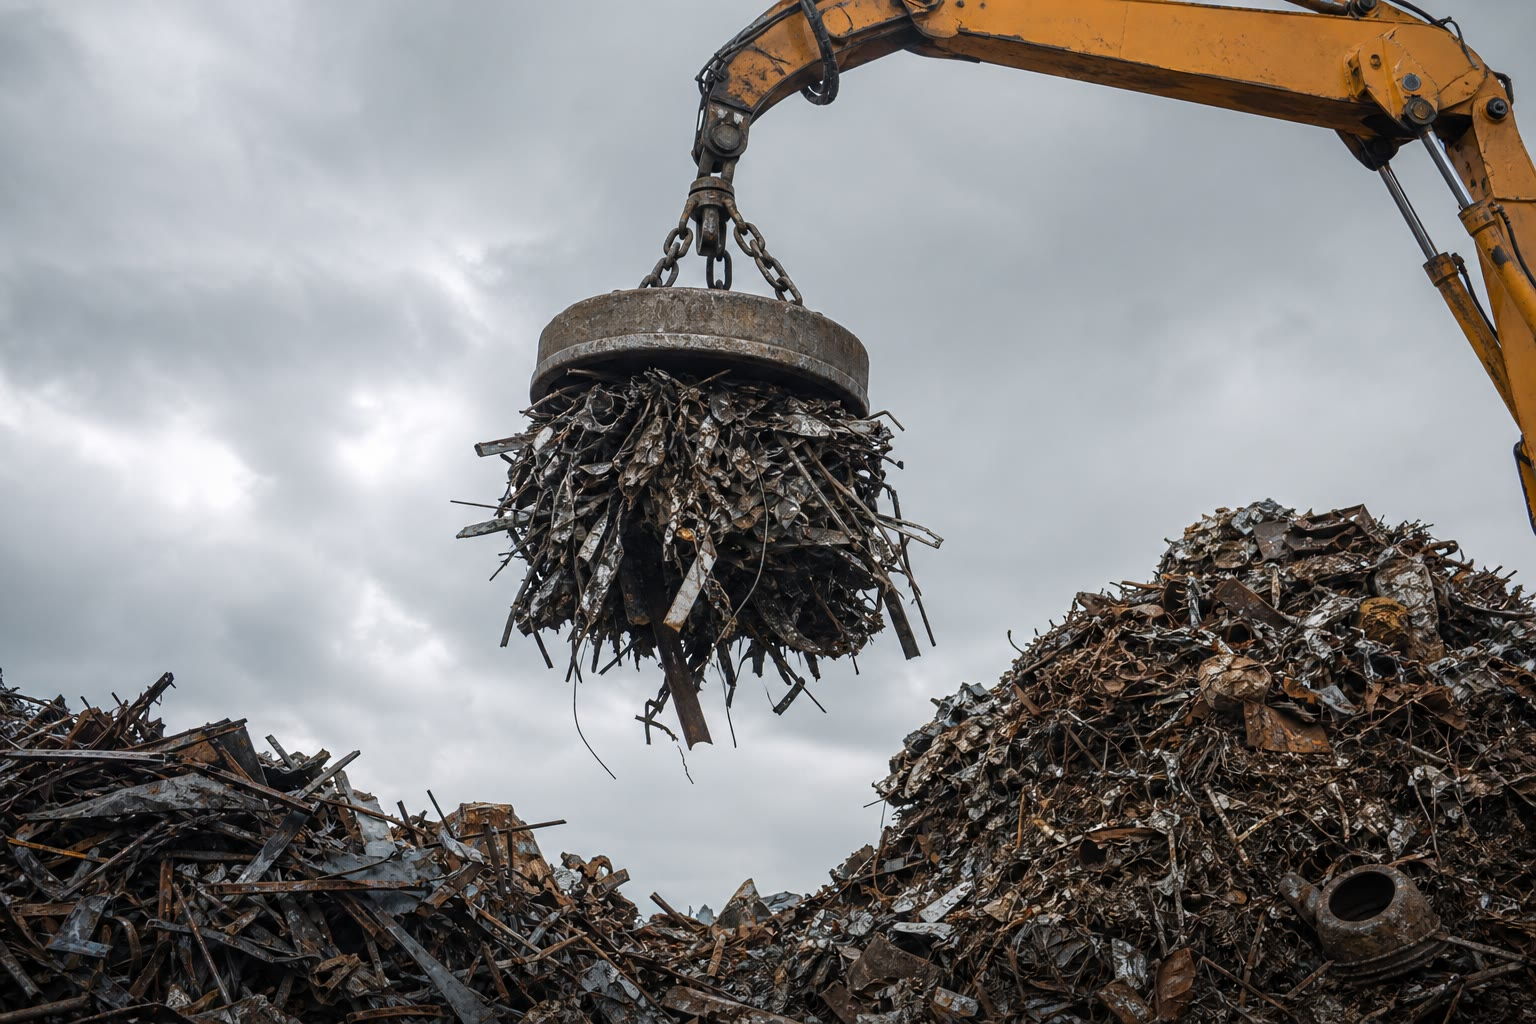
\includegraphics[width=0.58\linewidth]{images/book5/ai/b5-06-scrapyard-electromagnet.jpg}

{\small 周末问题的实际应用：铁芯线圈的磁场使废铁本身磁化，并可按指令释放——设计中由\omterm{def:b3:electromagnetism-in-matter:hysteresis}{磁滞}现象才变得有趣的，正是后一半。}
\end{omfigure}

\section{问题：废料场起重器}

\begin{problem}\label{pb:b3:electromagnetism-in-matter:1}
\emph{废料场起重器。}一家回收场订购一台起重电磁铁：
一个平面极面的铁罐，直径一米，须能
吊起两吨重的压扁汽车压块，然后——同样重要——
\emph{按指令放下}它们。你是设计工程师。

\medskip\noindent\textbf{第一部分——为何用铁。}

\begin{enumerate}
  \item 裸线圈：400 匝，载流 \qty{25}{A}，分布于
        一条长约 $\sim\qty{1}{m}$ 的磁路上。估算无铁时的 $B \sim
        \mu_0NI/\ell$。
  \item 用两句话，结合\omterm{def:b3:electromagnetism-in-matter:hysteresis}{磁畴}解释为何在线圈中填入铁芯，
        会使该值增大约 $\sim\mu_{\text{r}}$ 倍。
  \item 铁的\omterm{def:b3:electromagnetism-in-matter:magnetisation}{磁化强度}在 $M_{\text{s}} \approx
        \qty{1.7e6}{A/m}$ 时饱和。计算它对极面场所设的上限 $\mu_0M_{\text{s}}$，
        无论线圈如何工作。
  \item 每个铁原子贡献 $\approx 2.2$ 个\omterm{prop:b3:quantum-angular-momentum:magnetic}{玻尔磁子}。
        检验：取 $n = \qty{8.5e28}{m^{-3}}$，
        由此推算 $M_{\text{s}}$。
  \item 为何极面须经机械加工而平整，并保持
        无锈迹与砂粒？（见
        \cref{ex:b3:electromagnetism-in-matter:electromagnet}。）
  \item 负载本身也成为磁路的一部分。
        画出磁通路径：磁罐芯、北极面、钢制压块、
        南极面，再经磁轭返回。
\end{enumerate}

\medskip\noindent\textbf{第二部分——磁路与作用力。}

\begin{enumerate}[resume]
  \item 建立磁路模型：铁芯路径 $\ell = \qty{1.2}{m}$，
        $\mu_{\text{r}} = 2000$，两处等效气隙
        （极面–压块接触处）各 $e = \qty{1.5}{mm}$。写出
        $H$ 沿回路的安培环路定理。
  \item 计算单位面积上的三项磁阻项
        （$\ell/\mu_{\text{r}}$ 与 $2e$ 相比），并说明
        毫米量级的气隙仍占用了线圈的大部分磁动势。
  \item 取 $NI = \num{10000}$ 安匝，计算
        气隙中的 $B$。
  \item 每个极面上的提升压强为 $B^2/2\mu_0$
        （即每接近一米所释放的磁能密度）。
        对所得 $B$ 以 \unit{kPa} 为单位求值。
  \item 极面总面积 $A = \qty{0.12}{m^2}$，计算
        提升力，并换算为吨。
  \item 能否以二倍裕量满足两吨的设计指标？
        若不能，调整 $NI$ 并给出新的电流值。
  \item 压块可能仅约三分之一的面积与极面接触，
        且等效气隙更宽。重新计算以下条件下的力：
        $e = \qty{4}{mm}$，$A_{\text{有效}} = \qty{0.04}{m^2}$，
        并说明为何额定起重量以“平板”工况下的承载能力标注。
\end{enumerate}

\medskip\noindent\textbf{第三部分——记住与遗忘。}

\begin{enumerate}[resume]
  \item 场地拨动开关以放下压块——压块却仍吸住不放。
        请结合\omterm{def:b3:electromagnetism-in-matter:hysteresis}{磁滞回线}指出其原因。
  \item 为何磁罐必须采用\emph{软}铁（
        $H_{\text{c}}$ 小、$B_{\text{r}}$ 小）而非
        硬磁钢？
  \item 即便是软铁，仍保留少量\omterm{def:b3:electromagnetism-in-matter:hysteresis}{剩磁}。请提出
        标准的消除方法：施加短暂的\emph{反向}电流脉冲——
        该脉冲所指向的是\omterm{def:b3:electromagnetism-in-matter:hysteresis}{磁滞回线}上的哪一点？
  \item 某些控制器则改施衰减的交变电流。
        画出 $B$--$H$ 轨迹的变化情况，并说明
        为何它最终处于退磁状态。
  \item 该起重机还需直接吊运刚从熔炉取出的热板坯，
        温度为 \qty{800}{\celsius}。铁的居里点为
        \qty{1043}{K}：提升力会发生什么变化？原因何在？
        （见\cref{thm:b3:phase-transitions:meanfield}。）
  \item 一名夏季实习生建议，通过将气隙加倍、
        并将 $NI$ 加倍来节省铜材。请用第二部分的公式
        解释这种不对称性：哪一项减半，哪一项
        仅仅保持不变？
\end{enumerate}

\medskip\noindent\textbf{第四部分——功率、热量与费用。}

\begin{enumerate}[resume]
  \item 线圈：400 匝铜线，平均匝长
        \qty{2.5}{m}，导线\omterm{def:b3:scattering-theory:cross-section}{截面}积 \qty{16}{mm^2}，电阻率
        $\rho = \qty{1.7e-8}{\ohm.m}$。计算其电阻。
  \item 当 $I = \qty{25}{A}$ 时，求耗散功率，以及
        以 \qty{60}{\percent} 占空比工作八小时班次的每日能耗。
  \item 两气隙中所储存的磁能
        （$B^2/2\mu_0 \times$ 体积）：计算该值，并与
        线圈一\emph{秒}内的耗散能量相比较。其余的电能
        去向何处？
  \item 放下负载时，几乎没有存储的能量回馈给电网。
        试结合回线面积与
        感应尖峰，说明为何控制器需要
        在线圈两端设置续流（反激）通路。
  \item 悬吊压块时若突然断电，压块会怎样？
        \omterm{def:b3:electromagnetism-in-matter:hysteresis}{剩磁}\emph{单独}能维持什么？论证
        场地“任何人不得在通电磁铁下方行走”的规定——
        以及电池备份式起重机的销售宣传。
  \item 用四句话概括本设计：磁场上限由 $M_{\text{s}}$ 决定，
        作用力由 $B^2A/2\mu_0$ 决定，可控性由软铁\omterm{def:b3:electromagnetism-in-matter:hysteresis}{磁滞}决定，
        运行成本由 $RI^2$ 决定——整章内容
        都系于这一台起重机之上。
\end{enumerate}
\end{problem}
